\section{Muhammad Reza Syachrani - 1174084}
\subsection{Teori}
\begin{enumerate}

	\item Jelaskan kenapa file suara harus di lakukan MFCC. dilengkapi dengan ilustrasi atau gambar
	\hfill\\
digunakan untuk mendapatkan nilai dari vektor suara tersebut yang berguna untuk mendapatkan suatu parameter dan informasi mengenai ciri dari suara.
\begin{figure}[H]
    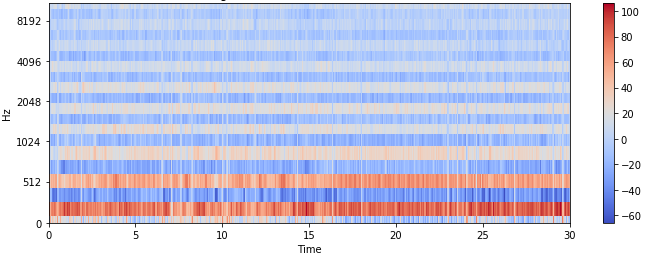
\includegraphics[width=12cm]{figures/1174084/6/teori1.png}
    \centering
    \caption{Teori 1}
\end{figure}

\item Jelaskan konsep dasar neural network.dilengkapi dengan ilustrasi atau gambar.
	\hfill\\
	Konsep dasar neural network sendiri di mulai dari ide dasar neural network otak manusia, dimana otak terdiri dari neuron, neuron ini berfungsi memproses setiap informasi yang masuk. Satu neuron memiliki satu akson dan minimal satu dendrit. sehingga konsep dasar ini membangun neural network buatan yang disebut (Artificial Neural Network).

\begin{figure}[H]
    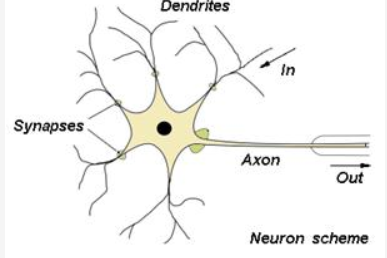
\includegraphics[width=12cm]{figures/1174084/6/teori2.png}
    \centering
    \caption{Teori 2}
\end{figure}

\item Jelaskan konsep pembobotan dalam neural network.dilengkapi dengan ilustrasi atau gambar
	\hfill\\
	Konsep pembobotan dalam neural network menggunakan algoritma backpropagation untuk memperkecil tingkat eror dengan menyesuaikan nilai bobot berdasarkan perbedaan output serta target yang diinginkan.
\begin{figure}[H]
    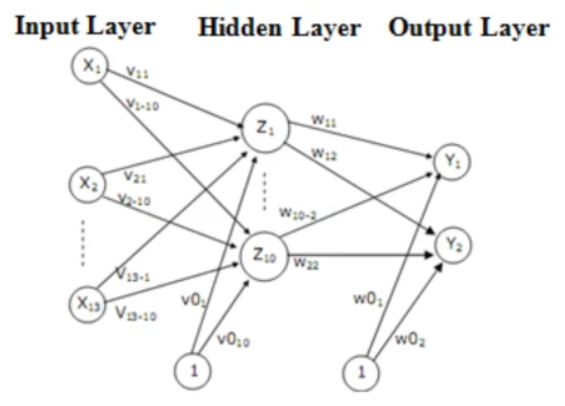
\includegraphics[width=12cm]{figures/1174084/6/teori3.png}
    \centering
    \caption{Teori 3}
\end{figure}

\item Jelaskan konsep fungsi aktifasi dalam neural network. dilengkapi dengan ilustrasi atau gambar
\hfill\\
	merupakan fungsi matematis yang digunakan untuk mendapatkan output neuron dari nilai inputnya. Disebut suatu aktivasi karena output akan bernilai jika dapat melampaui nilai threshold-nya.
\begin{figure}[H]
    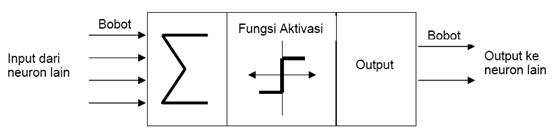
\includegraphics[width=8cm]{figures/1174084/6/teori4.png}
    \centering
    \caption{Teori 4}
\end{figure}

\item Jelaskan cara membaca hasil plot dari MFCC,dilengkapi dengan ilustrasi atau gambar.
	\hfill\\
Dapat dilakukan dengan sampel  suara  pengguna diubah dalam  bentuk  file  *.wav  yang  digunakan  sebagai  inputan kemudian direpresentasikan menjadi sinyal suara dalam bentuk matriks dengan menggunakan perintah auudiread di Matlab R2017a. hasil sampel suara pada gambar dibawah.
\begin{figure}[H]
    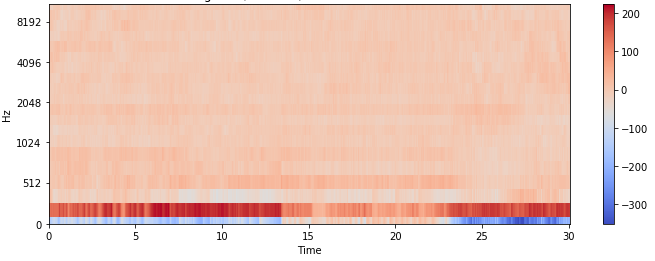
\includegraphics[width=8cm]{figures/1174084/6/teori5.png}
    \centering
    \caption{Teori 5}
\end{figure}

\item Jelaskan apa itu one-hot encoding,dilengkapi dengan ilustrasi kode dan atau gambar.
	\hfill\\
	proses dimana variabel kategorikal dikonversi menjadi bentuk yang dapat disediakan untuk algoritma ML untuk melakukan pekerjaan yang lebih baik dalam prediksi.
\begin{figure}[H]
    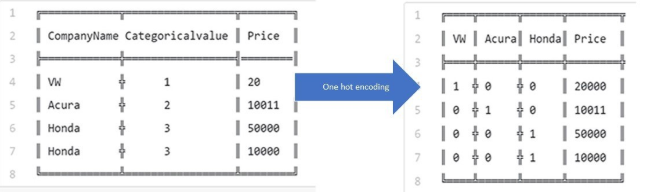
\includegraphics[width=8cm]{figures/1174084/6/teori6.png}
    \centering
    \caption{Teori 6}
\end{figure}

\item Jelaskan apa fungsi dari np.unique dan to\_categorical dalam kode program,dilengkapi dengan ilustrasi atau gambar.
	\hfill\\
	np.unique digunakan untuk membuat array, sedangkan  to\_categorical digunakan untuk mengubah vektor kelas yang berupa integer ( number ) menjadi matrix kelas biner.
\begin{figure}[H]
    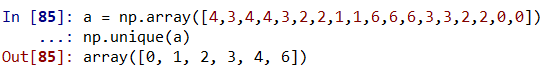
\includegraphics[width=8cm]{figures/1174084/6/teori7_1.png}
    \centering
    \caption{Teori 7}
\end{figure}

\begin{figure}[H]
    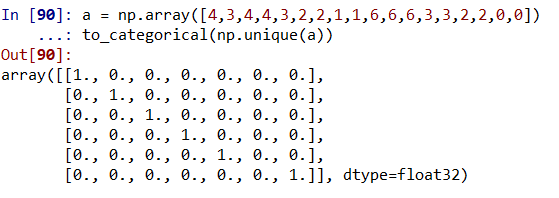
\includegraphics[width=8cm]{figures/1174084/6/teori7_2.png}
    \centering
    \caption{Teori 7}
\end{figure}

\item Jelaskan apa fungsi dari Sequential dalam kode program,dilengkapi dengan ilustrasi atau gambar.
	\hfill\\
	Sequential berfungsi sebagai tumpukan linear lapisan.
\begin{figure}[H]
    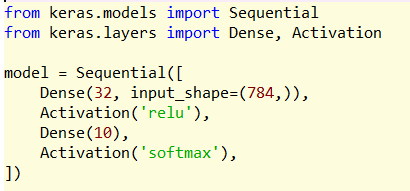
\includegraphics[width=8cm]{figures/1174084/6/teori8.png}
    \centering
    \caption{Teori 8}
\end{figure}
\end{enumerate}



\subsection{Praktek}
\begin{enumerate}


\item Jelaskan isi dari data GTZAN Genre Collection dan data dari freesound.
	\hfill\\
	 GTZAN Genre Collection berisikan klasifikasi genre musik. terdapat 10 genre musik didalamnya yaitu blues, clasisscal, country, disco, hiphop, jazz, metal, pop, reggae, dan rock. Dalam setiap genre tersebut berisikan 100 tracks musik.
\lstinputlisting[firstline=8, lastline=28]{src/1174084/6/1174084.py}	
	 

\item Jelaskan perbaris kode program dengan kata-kata dan dilengkapi ilustrasi gambar fungsi dari display mfcc() .
	\hfill\\

Ini spectogram dari lagu genre metal (source dari GTZAN Genre Collection).
\lstinputlisting[firstline=30, lastline=32]{src/1174084/6/1174084.py}
\begin{figure}[H]
	\centering
	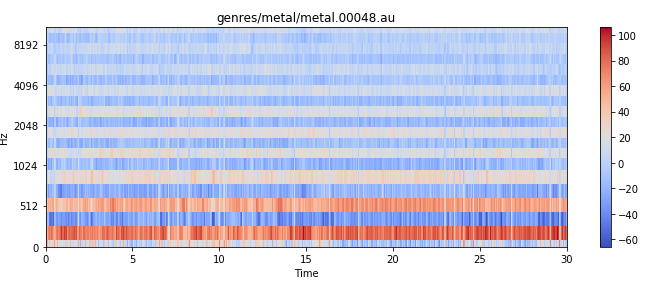
\includegraphics[width=10cm]{figures/1174084/6/1.png}
	\caption{spectogram dari lagu genre metal}
\end{figure}

Ini spectogram dari lagu genre classical (source dari GTZAN Genre Collection).
\lstinputlisting[firstline=33, lastline=35]{src/1174084/6/1174084.py}
\begin{figure}[H]
	\centering
	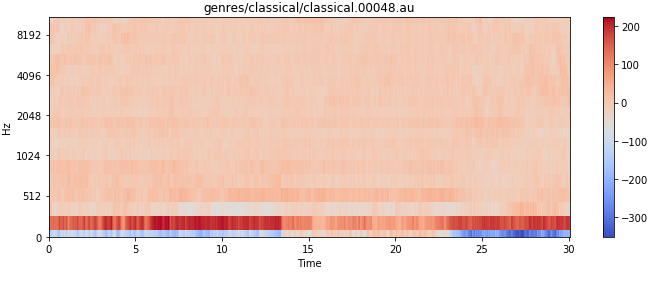
\includegraphics[width=10cm]{figures/1174084/6/2.png}
	\caption{spectogram dari lagu genre classical}
\end{figure}

Ini spectogram dari lagu genre pop (source dari GTZAN Genre Collection).
\lstinputlisting[firstline=36, lastline=38]{src/1174084/6/1174084.py}
\begin{figure}[H]
	\centering
	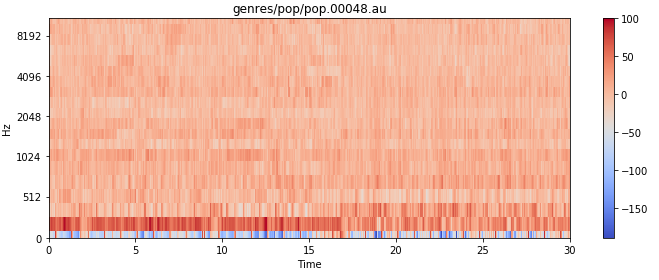
\includegraphics[width=10cm]{figures/1174084/6/3.png}
	\caption{spectogram dari lagu genre pop}
\end{figure}

Ini spectogram dari lagu genre reggae (source dari GTZAN Genre Collection).
\lstinputlisting[firstline=39, lastline=41]{src/1174084/6/1174084.py}
\begin{figure}[H]
	\centering
	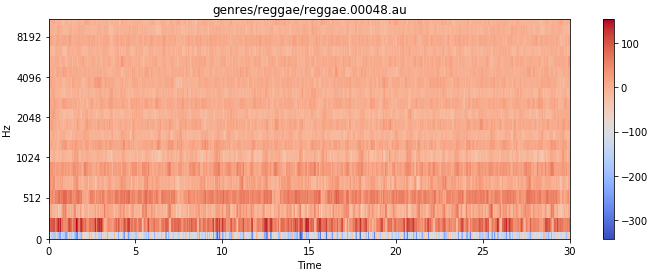
\includegraphics[width=10cm]{figures/1174084/6/4.png}
	\caption{spectogram dari lagu genre reggae}
\end{figure}

Ini spectogram dari lagu genre rock (source dari GTZAN Genre Collection).
\lstinputlisting[firstline=42, lastline=44]{src/1174084/6/1174084.py}
\begin{figure}[H]
	\centering
	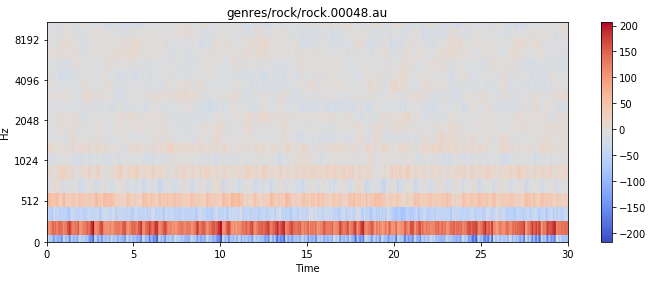
\includegraphics[width=10cm]{figures/1174084/6/5.png}
	\caption{spectogram dari lagu genre rock}
\end{figure}


\item Jelaskan perbaris kode program dengan kata-kata dan dilengkapi ilustrasi gambar fungsi dari extract features song()
	\hfill\\
	Mengapa mengambil 25000 row pertama? dikarenakan Audio yang terdapat pada dataset ini tidak menentu durasinya. Dan kita harus mengambil data yang memiliki durasi yang sama untuk mempermudah dalam melakukan training.
	
\lstinputlisting[firstline=45, lastline=53]{src/1174084/6/1174084.py}		
\begin{figure}[H]
    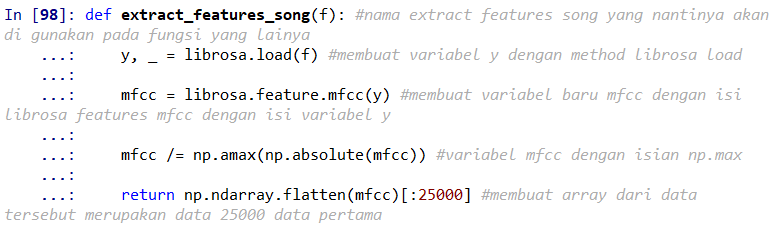
\includegraphics[width=8cm]{figures/1174084/6/6.png}
    \centering
    \caption{Praktek 3}
\end{figure}


\item Jelaskan perbaris kode program dengan kata-kata dan dilengkapi ilustrasi gambar fungsi dari generate features and labels().
	\hfill\\

\lstinputlisting[firstline=55, lastline=73]{src/1174084/6/1174084.py}
\begin{figure}[H]
    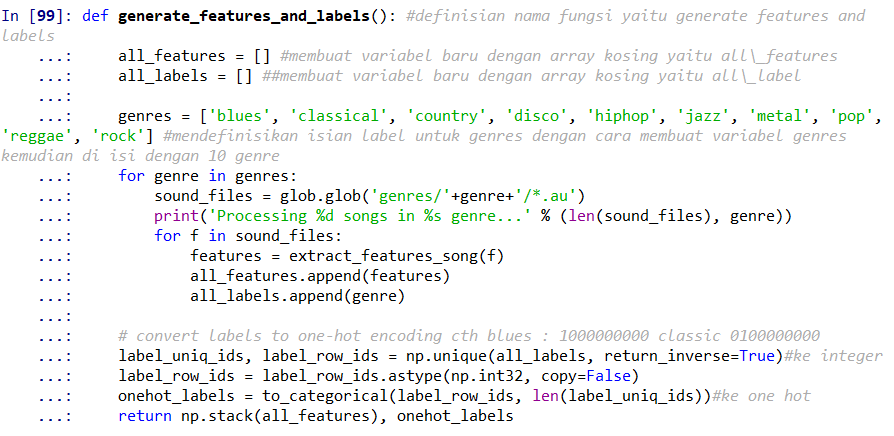
\includegraphics[width=8cm]{figures/1174084/6/7.png}
    \centering
    \caption{Praktek 4}
\end{figure}


\item Jelaskan dengan kata dan praktek kenapa penggunaan fungsi generate features and labels() sangat lama ketika meload dataset genre.
	\hfill\\
Karena mesin membaca file satu persatu yang ada pada folder dan dalam folder tersebut dan setiap folder terdapat 100 file sehingga menjadi lama dan mengolah data yang tadinya suara menjadi bentuk vektor.
\lstinputlisting[firstline=75, lastline=76]{src/1174084/6/1174084.py}
\begin{figure}[H]
    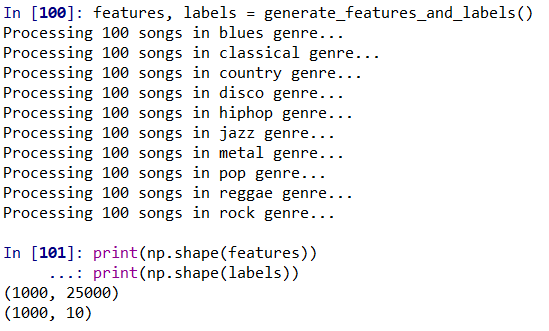
\includegraphics[width=8cm]{figures/1174084/6/8.png}
    \centering
    \caption{Praktek 5}
\end{figure}

\item  Jelaskan kenapa harus dilakukan pemisahan data training dan data set sebesar 80 persen? Praktekkan dengan kode dan Tunjukkan keluarannya
	\hfill\\
	Melakukan training split 80\% supaya mesin dapat terus belajar tentang data baru, jadi ketika prediksi dibuat tentang data yang terlatih itu bisa mendapatkan persentase yang cukup bagus.
\lstinputlisting[firstline=82, lastline=107]{src/1174084/6/1174084.py}
\begin{figure}[H]
    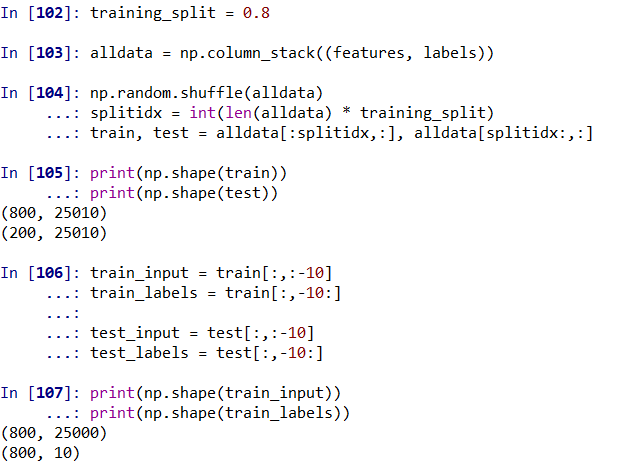
\includegraphics[width=12cm]{figures/1174084/6/9.png}
    \centering
    \caption{Praktek 6}
\end{figure}

\item Praktekkan dan jelaskan masing-masing parameter dari fungsi Sequential().
	\hfill\\
	Fungsi Sequential() ialah Sebuah model untuk menentukan izin pada setiap neuron, di sini adalah 100 dense yang merupakan 100 neuron pertama dari data pelatihan. Fungsi dari relay itu sendiri adalah untuk mengaktifkan neuron atau input yang memiliki nilai maksimum. Sedangkan untuk dense 10 itu adalah output dari hasil neuron yang telah berhasil diaktifkan, untuk dense 10 diaktifkan menggunakan softmax.
\lstinputlisting[firstline=109, lastline=115]{src/1174084/6/1174084.py}	
\begin{figure}[H]
    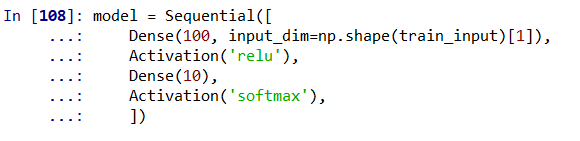
\includegraphics[width=8cm]{figures/1174084/6/10.png}
    \centering
    \caption{Praktek 7}
\end{figure}

\item  Praktekkan dan jelaskan masing-masing parameter dari fungsi compile().
	\hfill\\
	Model Compile di perjelas dengan gambar dibawah, Hasil output pada kode tersebut seperti gambar  menjelaskan bahwa dense pertama itu memiliki 100 neurons dengan parameter sekitar 2 juta lebih dengan aktviasi 100, jadi untuk setiap neurons memiliki masing-masing 1 aktivasi. Sama halnya seperti dense 2 memiliki jumlah neurons sebanyak 10 dengan parameter 1010 dan jumlah aktivasinya 10 untuk setiap neurons tersebut dan total parameternya sekitar 2.5 juta data yang akan dilatih pada mesin tersebut.
\lstinputlisting[firstline=117, lastline=121]{src/1174084/6/1174084.py}		
\begin{figure}[H]
    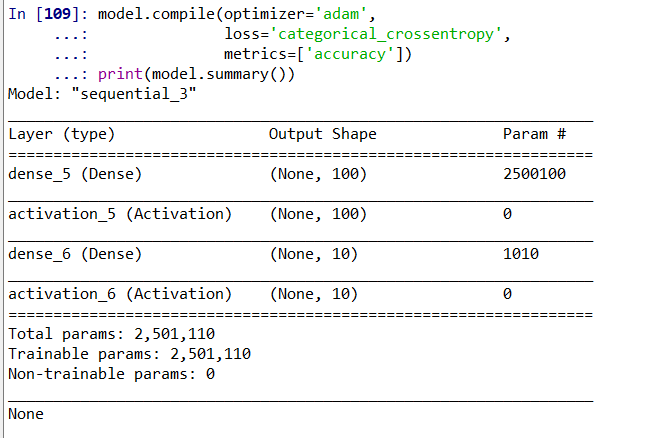
\includegraphics[width=8cm]{figures/1174084/6/11.png}
    \centering
    \caption{Praktek 8}
\end{figure}

\item  Praktekkan dan jelaskan masing-masing parameter dari fungsi fit().
	\hfill\\
	Kode tersebut berfungsi untuk melatih mesin dengan data training input dan training label. Epochs ini merupakan iterasi atau pengulangan berapa kali data tersebut akan dilakukan. Batch\_size ini adalah jumlah file yang akan dilakukan pelatihan pada setiap 1 kali pengulangan. Sedangkan validation\_split itu untuk menentukan presentase dari cross validation atau k-fold sebanyak 20\% dari masing-masing data pengulangan.
\lstinputlisting[firstline=123, lastline=125]{src/1174084/6/1174084.py}	
\begin{figure}[H]
    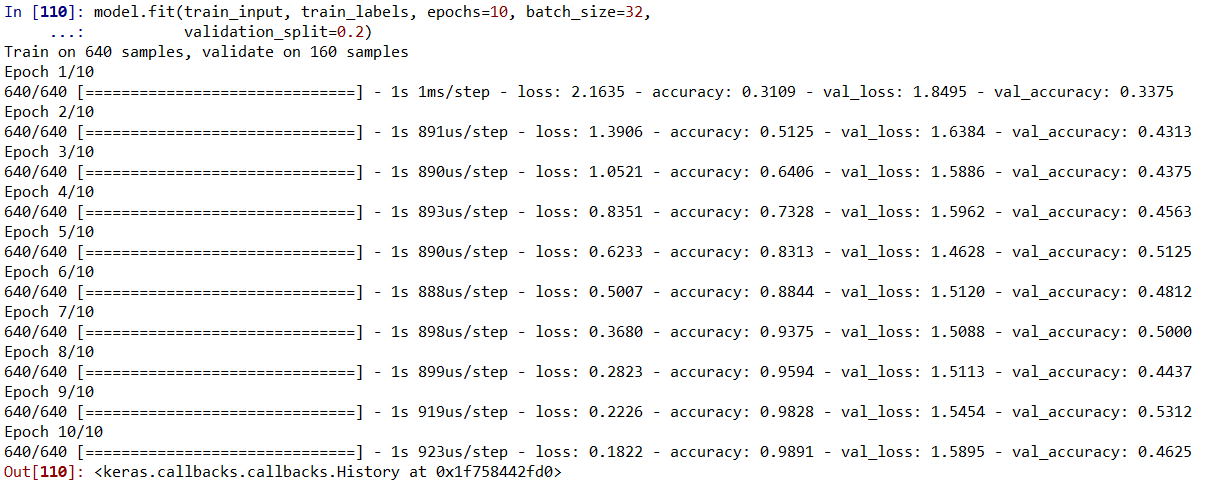
\includegraphics[width=8cm]{figures/1174084/6/12.png}
    \centering
    \caption{Praktek 9}
\end{figure}


\item Praktekkan dan jelaskan masing-masing parameter dari fungsi evaluate().
	\hfill\\
	Fungsi evaluate atau evaluasi ini ialah untuk menguji data pengujian setiap file. Di sini ada data yang hilang sebesar 1.6111 data, sedangkan untuk akurasinya sekitar 51\%.
\lstinputlisting[firstline=127, lastline=132]{src/1174084/6/1174084.py}	
\begin{figure}[H]
    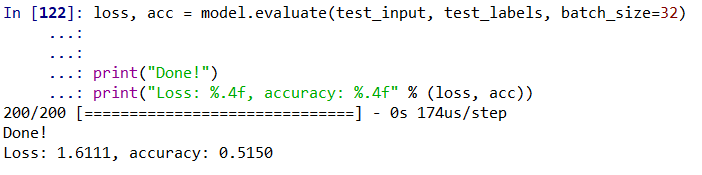
\includegraphics[width=8cm]{figures/1174084/6/13.png}
    \centering
    \caption{Praktek 10}
\end{figure}


\item Praktekkan dan jelaskan masing-masing parameter dari fungsi predict().
	\hfill\\
	Fungsi Predict ialah untuk menghasilkan suatu nilai yang sudah di prediksi dari data training sebelumnya. Gambar dibawah ini menjelaskan file yang di jalankan tersebut termasuk ke dalam genre apa, hasilnya bisa dilihat pada gambar tersebut presentase yang paling besar yakni genre classical. Maka lagu tersebut termasuk ke dalam genre classical dengan perbandingan presentase hasil prediksi.
\lstinputlisting[firstline=134, lastline=135]{src/1174084/6/1174084.py}	
\begin{figure}[H]
    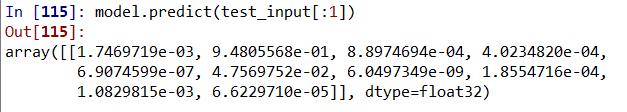
\includegraphics[width=8cm]{figures/1174084/6/14.png}
    \centering
    \caption{Praktek 11}
\end{figure}

\end{enumerate}


\subsection{Bukti Tidak Plagiat}
\begin{figure}[H]
	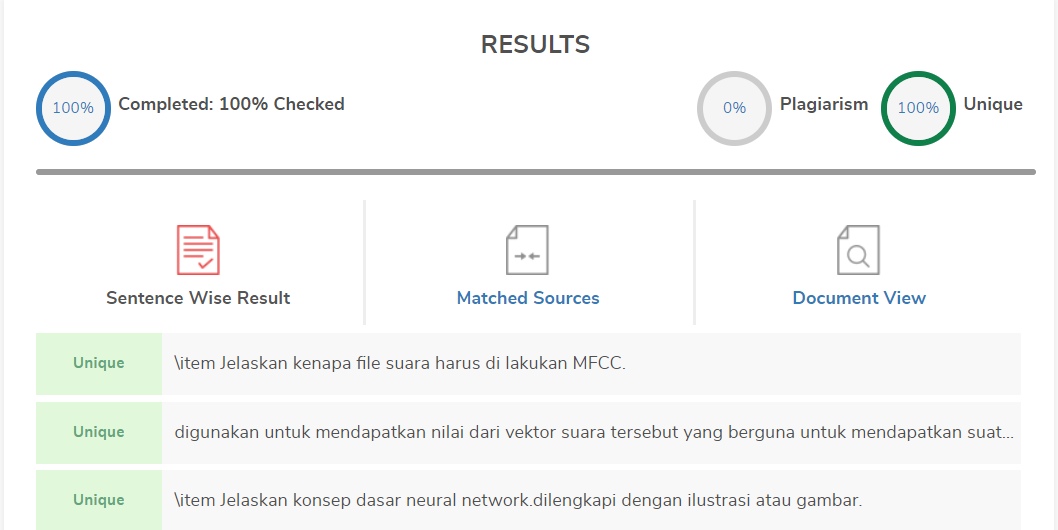
\includegraphics[width=4cm]{figures/1174084/6/plagiarism.png}
	\centering
	\caption{plagiarism}
\end{figure}


\subsection{Link Video Youtube}
https://youtu.be/MnrV7s-Tdy0

